\newapage
\chapter{Analiza wymagań}

\section{Diagramy}

\setlength{\parindent}{15pt}

\indent Diagram przypadków użycia jest narzędziem służącym do przedstawienia funkcjonalności systemu z punktu widzenia użytkownika.

\begin{figure}[H]
    \centering
    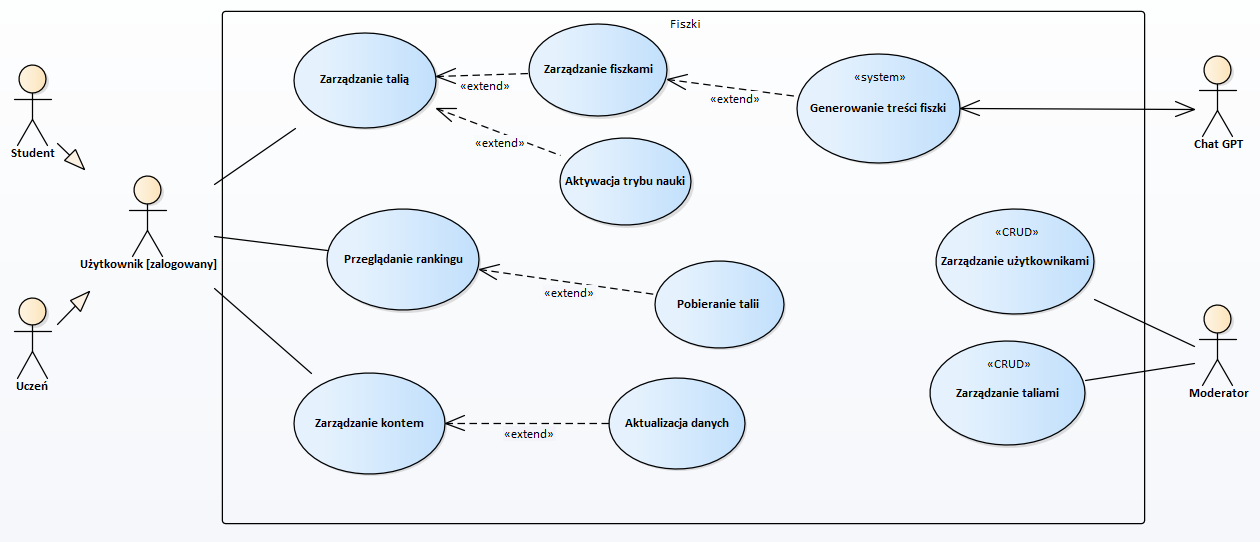
\includegraphics[width=1\textwidth]{chapters/chapter_6/diagram_przypadkow_uzycia}
    \caption{Diagram przypadków użycia.}
    \label{img:diagram_przypadkow_uzycia}
\end{figure}


\setlength{\parindent}{15pt}

\indent Diagram ERD (Entity-Relationship Diagram) to graficzne przedstawienie struktury bazy danych używane w projektowaniu i modelowaniu baz danych.



\begin{figure}[H]
    \centering
    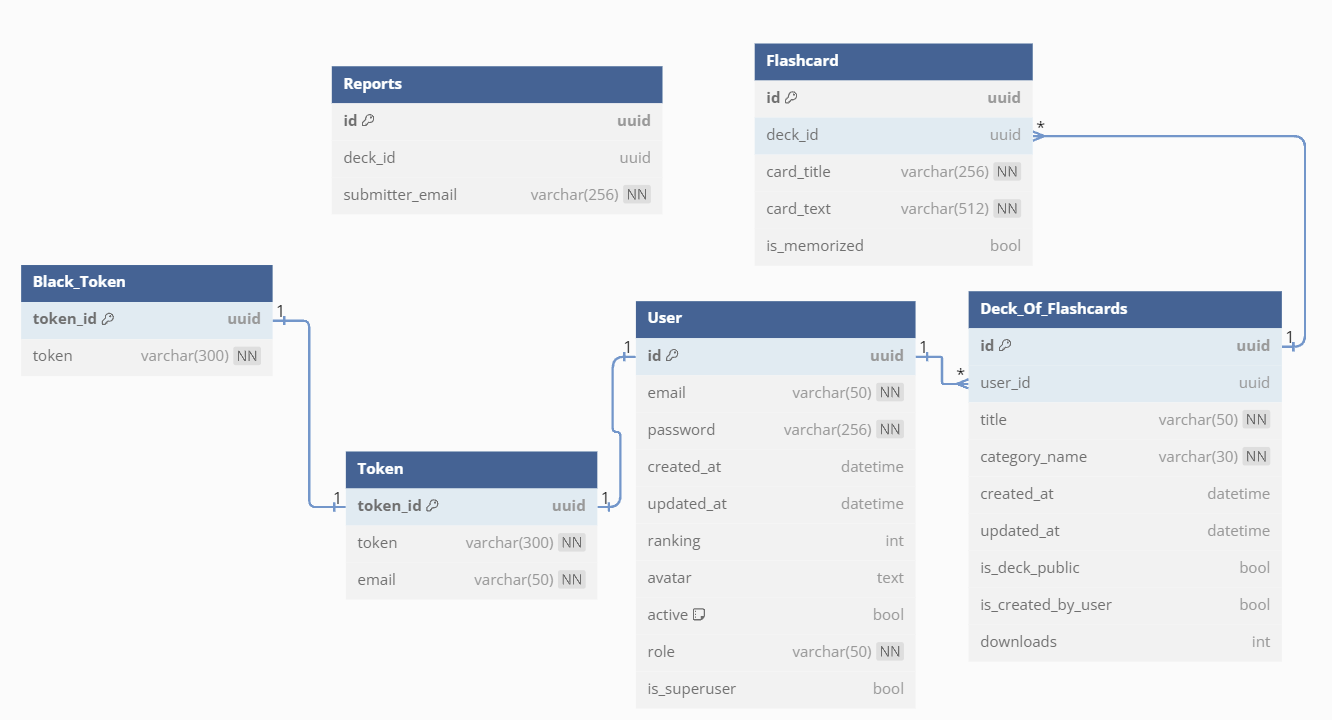
\includegraphics[width=1\textwidth]{chapters/chapter_6/erd}
    \caption{Diagram ERD.}
    \label{img:erd}
\end{figure}


\indent Diagram architektury stanowi reprezentację organizacji systemu informatycznego w oparciu o który został zrealizowany podjęty projekt.


\begin{figure}[H]
    \centering
    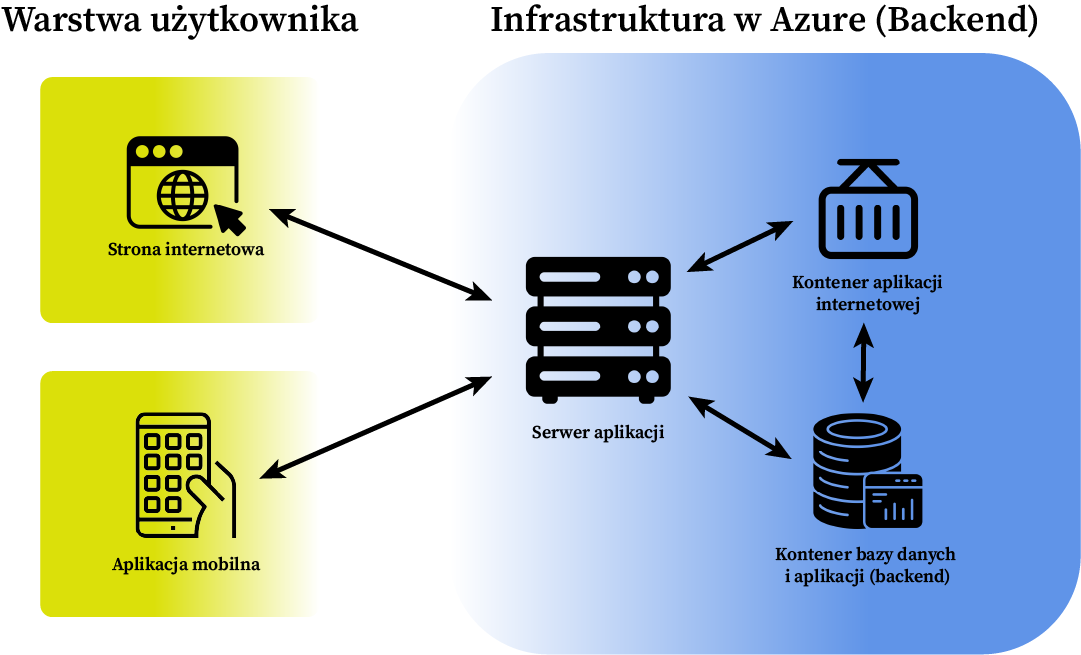
\includegraphics[width=0.6\textwidth]{chapters/chapter_6/diagram_architektury}
    \caption{Diagram architektury.}
    \label{img:diagram_architektury}
\end{figure}


\setlength{\parindent}{15pt}

\indent W diagramach sekwencji zostały przedstawione sposoby tworzenia deck’u oraz fiszk


\indent Użytkownik ma możliwość stworzyć deck dla siebie na dwa sposoby. Pierwszym sposobem  jest utworzenie go samodzielnie od podstaw, drugim jest pobranie talii udostępnionej przez innego użytkownika.
\begin{figure}[H]
    \centering
    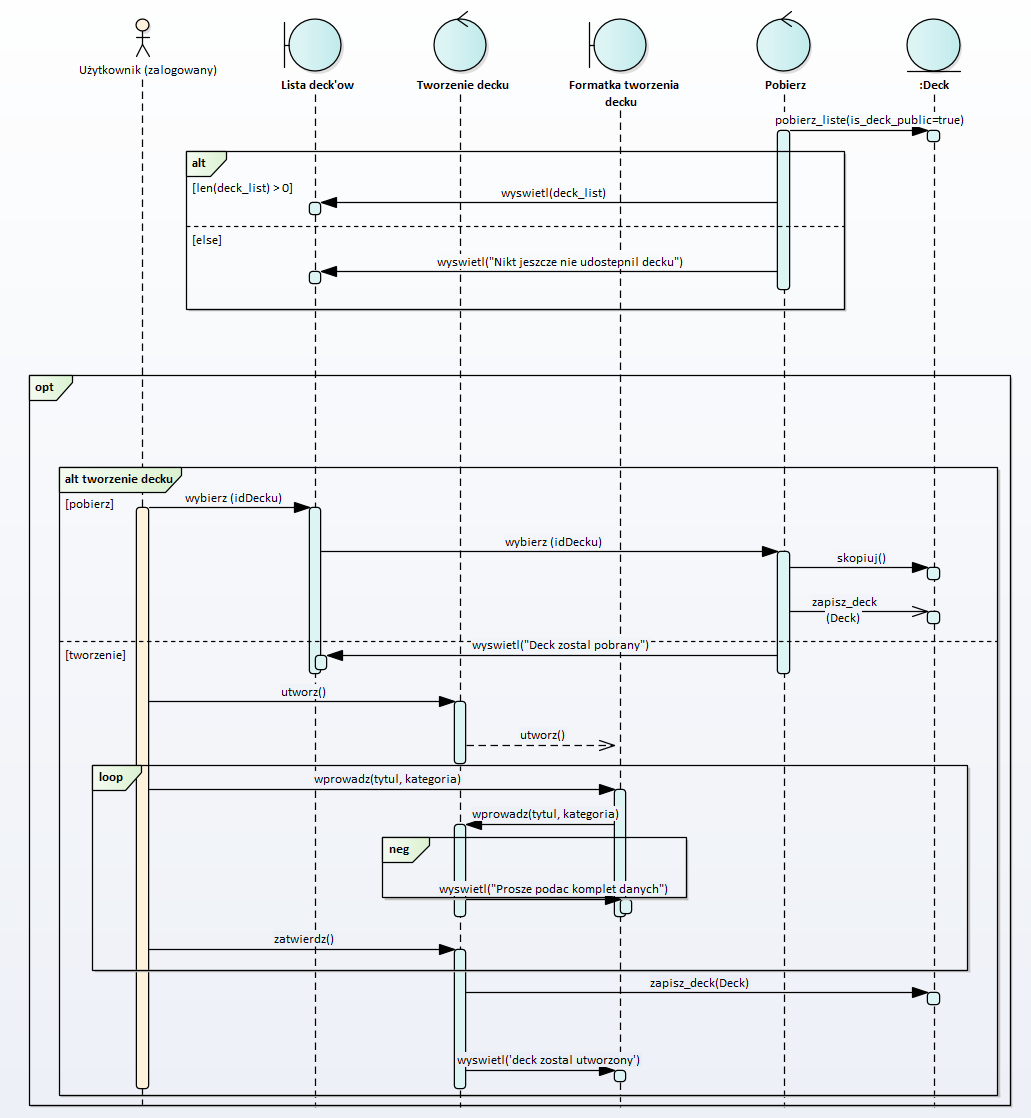
\includegraphics[width=1\textwidth]{chapters/chapter_6/diagram_sekwencji_1}
    \caption{Diagram sekwencji przdstawiający tworzenie talii fiszek.}
    \label{img:diagram_sekwencji_1}
\end{figure}

\indent Tworzenie fiszek natomiast może przebiec poprzez zredagowanie definicji zagadnienia samodzielnie (wpisaniu lub dyktowaniu przez mikrofon) lub wygenerowaniu jej za pomocą Chatu GPT.

    \begin{figure}[H]
    \centering
    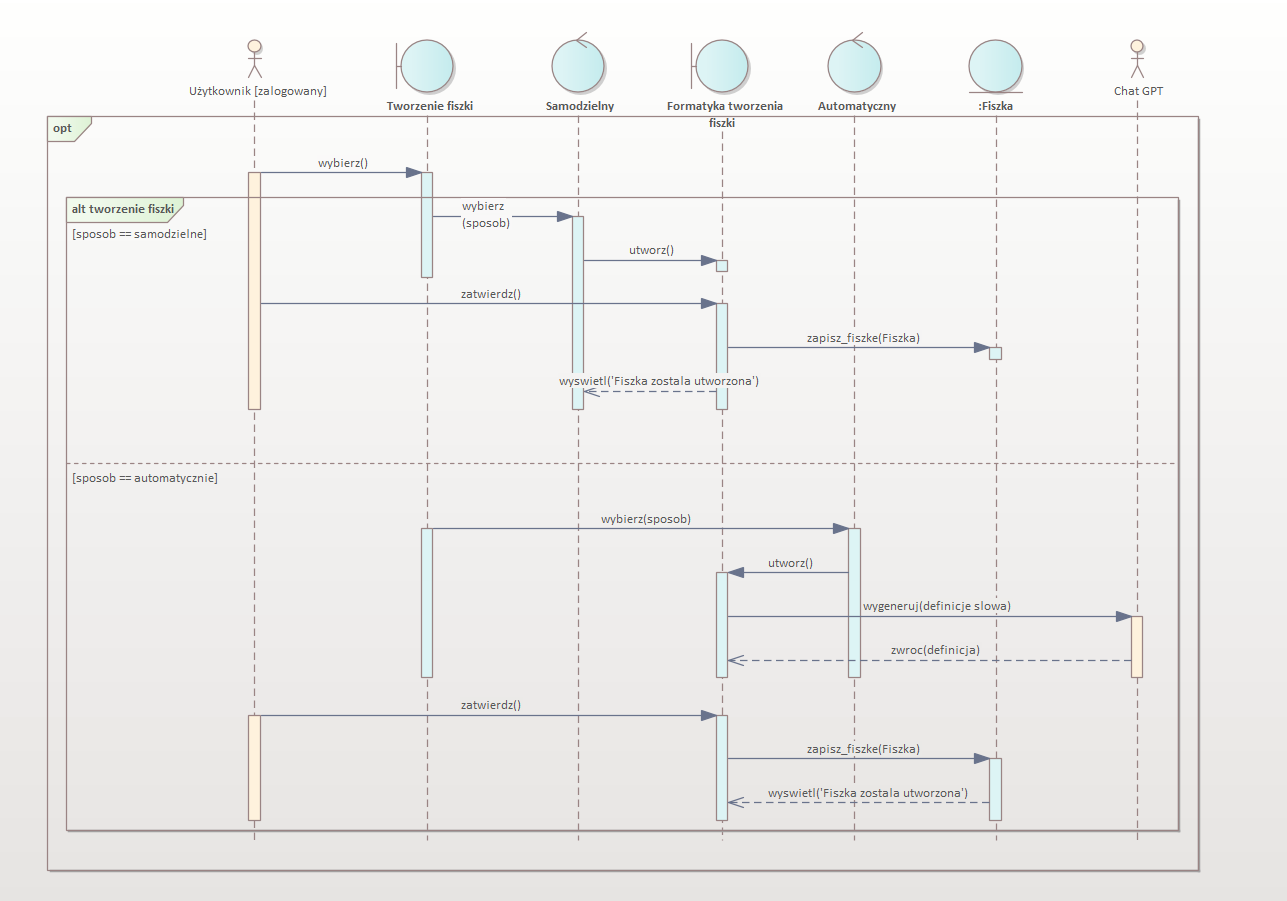
\includegraphics[width=1\textwidth]{chapters/chapter_6/diagram_sekwencji_2}
    \caption{Diagram sekwencji przestawiajacy tworzenie fiszki.}
    \label{img:diagram_sekwencji_2}
\end{figure}




    \setstretch{1}

    \section{Wymagania ogólne}

\subsection{Moduł autoryzacji}

    \begin{requirementstab}[label={tab:requirements:general},caption={Przykładowe wymaganie ogólne lub dziedzinowe}]
    \id{ WO1 }
    \priority{ M – must }
    \name{ Moduł autoryzacji }
    \descr{Rejestracja konta nowego użytkownika.
Możliwość usunięcia konta użytkownika.
Logowanie do systemu. Wylogowanie użytkownika z systemu.
Edycja danych użytkownika.
}
    \sholder{Zespół projektowy (UOB 01) \newline
Użytkownik systemu (UOB 03)
}
    \reqrelated{Rejestracja konta użytkownika (WF01) \newline
Logowanie do systemu (WF02) \newline
Wylogowanie z systemu (WF03) \newline
Edycja danych użytkownika (WF04) \newline
Usunięcie konta użytkownika (WF05) \newline
Weryfikacja konta użytkownika poprzez email  (WF14)
}

\end{requirementstab}

    \subsection{Moduł zarządzania talią}

\begin{requirementstab}[label={tab:requirements:deck},caption={Wymaganie ogólne dla modułu zarządzania talią}]
    \id{ WO2 }
    \priority{ M – must }
    \name{ Moduł zarządzania talią }
    \descr{Tworzenie talii fiszek. Pobranie talii utworzonej przez innych użytkowników. Edycja utworzonych talii fiszek lub edycja talii pobranej przez innych użytkowników. Usunięcie talii fiszek.}
    \sholder{Zespół projektowy (UOB 01) \newline
Użytkownik systemu (UOB 03)
}
    \reqrelated{Tworzenie talii fiszek (WF06) \newline
Usunięcie talii fiszek (WF07) \newline
Edycja talii fiszek (WF08) \newline
Import talii innych użytkowników (WF11)
}

\end{requirementstab}

    \subsection{Moduł uczenia}

\begin{requirementstab}[label={tab:requirements:learning},caption={Wymaganie ogólne dla modułu uczenia}]
    \id{ W03 }
    \priority{ M – must }
    \name{ Moduł uczenia }
    \descr{Tryb sterowania głosem pozwala na uruchomienie talii fiszek w specjalnym trybie, który pozwala na sterowanie talią fiszek przy wykorzystaniu komend głosowych. Zwykły tryb uczenia uruchamia talie w pełnym ekranie i pozwala na podzielenie talii na fiszki, które użytkownik zapamiętał i na te nie zapamiętane.}
    \sholder{Zespół projektowy (UOB 01) \newline
Użytkownik systemu (UOB 03)
}
    \reqrelated{Tryb uczenia się z talii fiszek (WF09) \newline
Sterowanie talią przy użyciu mowy (WF10)
}

\end{requirementstab}

    \subsection{Moduł udogodnień}

\begin{requirementstab}[label={tab:requirements:conveniences},caption={Wymaganie ogólne dla modułu udogodnień}]
    \id{ W04 }
    \priority{ S – should ) }
    \name{ Moduł udogodnień }
    \descr{Tryb dark mode i light mode pozwala użytkownikowi na zmianę kolorystyki systemy w celu uniknięcia przemęczenia wzroku. Kalendarz oznacza dni, w których użytkownik korzysta z aplikacji, może to spowodować większą motywację u użytkownika aby regularnie korzystał z systemu.}
    \sholder{Zespół projektowy (UOB 01) \newline
Użytkownik systemu (UOB 03)
}
    \reqrelated{Tryb dark mode i light mode (WF12) \newline
Kalendarz śledzący aktywność (WF13)
}

\end{requirementstab}

\subsection{Moduł wspomagania tworzenia talii}

\begin{requirementstab}[label={tab:requirements:deck_creation_support},caption={Wymaganie ogólne dla modułu wspomagania tworzenia talii}]
    \id{ W05 }
    \priority{ W – won’t }
    \name{ Moduł wspomagania tworzenia talii }
    \descr{Analiza dokumentów poprzez wykorzystanie sztucznej inteligencji pozwala na wygenerowanie zestawu fiszek poprzez wgranie do systemu dokumentu w formacie csv lub pdf. Użytkownik może wygenerować treść fiszki, podając kilka słów kluczowych na podstawie których sztuczna inteligencja przeszukuje bazę definicji i na podstawie wyszukanych definicji generuje treść.}
    \sholder{Użytkownik systemu (UOB 03)}
    \reqrelated{Tworzenie talii fiszek przez analizę dokumentu (WF15) \newline
Generowanie treści fiszki na podstawie słów kluczowych (WF16)
}

\end{requirementstab}

    \section{Wymagania funkcjonalne}

\subsection{Rejestracja konta użytkownika}

    \begin{requirementstab}[label={tab:requirements:user_registration},caption={Wymagania na interfejs z otoczeniem dla procesu rejestracji użytkownika}]
    \id{WF01}
    \priority{M – must}
    \name{Rejestracja nowego użytkownika w systemie}
    \descr{Użytkownik musi utworzyć konto aby móc korzystać z aplikacji.}
    \acceptcrit{Nowy użytkownik dodany do systemu}
    \inputdata{nickname, email, hasło}
    \preconditions{Użytkownik musi posiadać adres email}
    \postconditions{Utworzenie konta użytkownika}
    \exceptions{Brak łączności z bazą danych. Wprowadzenie dane przez użytkownika istnieją już w bazie danych.}
    \implementation{uzupełniane w trakcie sprintu – opis sposobu realizacji}
    \sholder{Zespół projektowy (UOB 01)
Użytkownik systemu (UOB 03) }
    \reqrelated{Logowanie do systemu (WF02) \newline
Wylogowanie z systemu (WF03) \newline
Edycja danych użytkownika (WF04) \newline
Usunięcie konta użytkownika (WF05) \newline
Weryfikacja konta użytkownika poprzez email (WF14)}
\end{requirementstab}

    \subsection{Logowanie do systemu}

\begin{requirementstab}[label={tab:requirements:system_login},caption={Wymagania na interfejs z otoczeniem dla procesu logowania do systemu}]
    \id{WF02}
    \priority{M – must}
    \name{Logowanie do systemu}
    \descr{Użytkownik musi zalogować się do systemu, aby mieć dostęp do systemu.}
    \acceptcrit{Pomyślne zalogowanie do systemu}
    \inputdata{email i hasło}
    \preconditions{Posiadane konto użytkownika, konto musi być aktywne.}
    \postconditions{Dostęp do systemu}
    \exceptions{Brak łączności z bazą danych. Wprowadzenie niepoprawnych danych logowania, co uniemożliwia zalogowanie do systemu.}
    \implementation{uzupełniane w trakcie sprintu – opis sposobu realizacji}
    \sholder{Zespół projektowy (UOB 01) }
    \reqrelated{Rejestracja konta użytkownika (WF01) \newline
Wylogowanie z systemu (WF03) \newline
Edycja danych użytkownika (WF04) \newline
Usunięcie konta użytkownika (WF05) \newline
Weryfikacja konta użytkownika poprzez email (WF14)}
\end{requirementstab}

    \subsection{Wylogowanie z systemu}

\begin{requirementstab}[label={tab:requirements:system_logout},caption={Wymagania na interfejs z otoczeniem dla procesu wylogowania z systemu}]
    \id{WF03}
    \priority{M – must}
    \name{Wylogowanie z systemu}
    \descr{Jako użytkownik chciałbym mieć możliwość wylogowania z systemu, aby inne osoby nie mogły korzystać z mojego konta.}
    \acceptcrit{Wylogowanie użytkownika z systemu.}
    \inputdata{Brak}
    \preconditions{Użytkownik zalogowany do systemu}
    \postconditions{Wylogowanie z systemu}
    \exceptions{Awaria bazy danych lub brak połączenia z bazą.}
    \implementation{uzupełniane w trakcie sprintu – opis sposobu realizacji}
    \sholder{Użytkownik systemu (UOB 03) }
    \reqrelated{Rejestracja konta użytkownika (WF01) \newline
Logowanie do systemu (WF02) \newline
Edycja danych użytkownika (WF04) \newline
Usunięcie konta użytkownika (WF05) \newline
Weryfikacja konta użytkownika poprzez email (WF14)}
\end{requirementstab}

    \subsection{Edycja danych użytkownika}

\begin{requirementstab}[label={tab:requirements:user_data_edit},caption={Wymagania na interfejs z otoczeniem dla procesu edycji danych użytkownika}]
    \id{WF04}
    \priority{M – must}
    \name{Edycja danych użytkownika}
    \descr{Jako użytkownik muszę mieć możliwość zmiany hasła lub email ponieważ mogę stracić dostęp do konta email lub moje hasło z różnych powodów może stać się jawne.}
    \acceptcrit{Zmienione parametry logowania}
    \inputdata{Użytkownik podaje nowy parametr wraz z hasłem, w celu edycji danych użytkownika}
    \preconditions{Posiadane konto użytkownika, użytkownik zalogowany do systemu.}
    \postconditions{Zmienione parametry logowania}
    \exceptions{Awaria bazy danych lub brak połączenia z bazą. Wprowadzenie niepoprawnych danych co uniemożliwia zmianę parametrów użytkownika.}
    \implementation{uzupełniane w trakcie sprintu – opis sposobu realizacji}
    \sholder{Użytkownik systemu (UOB 03) }
    \reqrelated{Rejestracja konta użytkownika (WF01) \newline
Logowanie do systemu (WF02) \newline
Wylogowanie z systemu (WF03) \newline
Usunięcie konta użytkownika (WF05) \newline
Weryfikacja konta użytkownika poprzez email (WF14)}
\end{requirementstab}

    \subsection{Usunięcie konta użytkownika}

\begin{requirementstab}[label={tab:requirements:user_account_deletion},caption={Wymagania na interfejs z otoczeniem dla procesu usunięcia konta użytkownika}]
    \id{WF05}
    \priority{M – must}
    \name{Usunięcie konta użytkownika}
    \descr{Jako użytkownik chcę mieć możliwość usunięcia swojego konta, gdy przestanę korzystać z aplikacji.}
    \acceptcrit{Usunięte konto użytkownika}
    \inputdata{email i hasło}
    \preconditions{Posiadane konto użytkownika, użytkownik zalogowany do systemu.}
    \postconditions{Konto użytkownika usunięte z systemu}
    \exceptions{Awaria bazy danych lub brak połączenia z bazą. Wprowadzenie niepoprawnych danych, co uniemożliwia usunięcie konta użytkownika.}
    \implementation{uzupełniane w trakcie sprintu – opis sposobu realizacji}
    \sholder{Użytkownik systemu (UOB 03) }
    \reqrelated{Rejestracja konta użytkownika (WF01) \newline
Logowanie do systemu (WF02) \newline
Wylogowanie z systemu (WF03) \newline
Edycja danych użytkownika (WF04) \newline
Weryfikacja konta użytkownika poprzez email (WF14)}
\end{requirementstab}

    \subsection{Tworzenie talii fiszek}

\begin{requirementstab}[label={tab:requirements:deck_creation},caption={Wymagania na interfejs z otoczeniem dla procesu tworzenia talii fiszek}]
    \id{WF06}
    \priority{M – must}
    \name{Tworzenie talii fiszek}
    \descr{Jako użytkownik muszę mieć możliwość utworzenia własnej talii fiszek, w celu uczenia się zagadnień, które mają dla mnie znaczenie.}
    \acceptcrit{Utworzona talia fiszek}
    \inputdata{tytuł talii fiszek, kategoria talii, tytuł fiszki, treść fiszki}
    \preconditions{Posiadane konto użytkownika, użytkownik zalogowany do systemu.}
    \postconditions{Utworzona nowa talia fiszek.}
    \exceptions{Awaria bazy danych lub brak połączenia z bazą. Puste pole z nazwą talii uniemożliwia tworzenie talii. Pusty tytuł fiszki lub pusta treść uniemożliwia utworzenie fiszki.}
    \implementation{uzupełniane w trakcie sprintu – opis sposobu realizacji}
    \sholder{Użytkownik systemu (UOB 03) }
    \reqrelated{Usunięcie talii fiszek (WF07) \newline
Edycja talii fiszek (WF08) \newline
Import talii innych użytkowników (WF11)}
\end{requirementstab}

\subsection{Usunięcie talii fiszek}

\begin{requirementstab}[label={tab:requirements:deck_deletion},caption={Wymagania na interfejs z otoczeniem dla procesu usunięcia talii fiszek}]
    \id{WF07}
    \priority{M – must}
    \name{Usunięcie talii fiszek}
    \descr{Jako użytkownik chcę mieć możliwość usunięcia talii fiszek, z których nie będę już korzystał.}
    \acceptcrit{Usunięta talia fiszek}
    \inputdata{Brak}
    \preconditions{Posiadane konto użytkownika, użytkownik zalogowany do systemu. Utworzona talia fiszek, którą można usunąć.}
    \postconditions{Talia fiszek zostaje usunięta.}
    \exceptions{Awaria bazy danych lub brak połączenia z bazą.}
    \implementation{uzupełniane w trakcie sprintu – opis sposobu realizacji}
    \sholder{Użytkownik systemu (UOB 03) }
    \reqrelated{Tworzenie talii fiszek (WF06) \newline
Edycja talii fiszek (WF08) \newline
Import talii innych użytkowników (WF11)}
\end{requirementstab}

    \subsection{Edycja talii fiszek}

\begin{requirementstab}[label={tab:requirements:deck_edit},caption={Wymagania na interfejs z otoczeniem dla procesu edycji talii fiszek}]
    \id{WF08}
    \priority{M – must}
    \name{Edycja talii fiszek}
    \descr{Jako użytkownik chcę mieć możliwość edycji talii fiszek, aby zaktualizować informacje dotyczące talii.}
    \acceptcrit{Zaktualizowana zawartość talii}
    \inputdata{Nowy tytuł talii, kategoria lub zmieniona treść fiszki.}
    \preconditions{Talia fiszek, która będzie edytowana.}
    \postconditions{Talia fiszek zostaje zaktualizowana o nowe informacje.}
    \exceptions{Awaria bazy danych lub brak połączenia z bazą. Puste pole dotyczące tytułu talii uniemożliwia zapisanie zmian.}
    \implementation{uzupełniane w trakcie sprintu – opis sposobu realizacji}
    \sholder{Użytkownik systemu (UOB 03) }
    \reqrelated{Tworzenie talii fiszek (WF06) \newline
Usunięcie talii fiszek (WF07) \newline
Import talii innych użytkowników (WF11)}
\end{requirementstab}

    \subsection{Tryb uczenia się z talii fiszek}

\begin{requirementstab}[label={tab:requirements:learning_mode},caption={Wymagania na interfejs z otoczeniem dla trybu uczenia się z talii fiszek}]
    \id{WF09}
    \priority{M – must}
    \name{Tryb uczenia się z talii fiszek}
    \descr{System musi posiadać tryb uczenia się, który pozwoli użytkownikowi na naukę i zapamiętywanie zagadnień znajdujących się w talii fiszek. W trakcie nauki użytkownik dzieli talię na zestaw z pojęciami które już opanował i na te, których jeszcze nie pamięta.}
    \acceptcrit{Talia fiszek zostaje podzielona na dwa zbiory, fiszki zapamiętane i nie zapamiętane.}
    \inputdata{Brak}
    \preconditions{Utworzona talia fiszek lub pobrana talia fiszek, która zostanie wykorzystana do nauki.}
    \postconditions{Talia fiszek zostaje podzielona na dwa zbiory, fiszki zapamiętane i nie zapamiętane.}
    \exceptions{Awaria bazy danych lub brak połączenia z bazą.}
    \implementation{uzupełniane w trakcie sprintu – opis sposobu realizacji}
    \sholder{Zespół projektowy (UOB 01) }
    \reqrelated{Sterowanie talią przy użyciu mowy (WF10)}
\end{requirementstab}

    \subsection{Sterowanie talią przy użyciu mowy}

\begin{requirementstab}[label={tab:requirements:voice_control},caption={Wymagania na interfejs z otoczeniem dla sterowania talią przy użyciu mowy}]
    \id{WF10}
    \priority{M – must}
    \name{Sterowanie talią przy użyciu mowy}
    \descr{Jako użytkownik chcę mieć możliwość uczenia się w warunkach, w których odczytywanie treści fiszki jest utrudnione, na przykład w trakcie prowadzenia samochodu. Sterowanie talią z przy użyciu mowy i odczytanie zawartości fiszki przez sztuczną inteligencję pozwala na naukę podczas prowadzenia pojazdu.}
    \acceptcrit{Użytkownik steruje talią fiszek przy użyciu komend głosowych}
    \inputdata{Brak}
    \preconditions{Utworzona talia fiszek}
    \postconditions{Talia fiszek pozostaje niezmieniona}
    \exceptions{Awaria bazy danych lub brak połączenia z bazą danych. Hałas, który aplikacja może przechwytywać, przez co komendy głosowe mogą działać niepoprawnie. Fiszki utworzone w innym języku niż angielski co może spowodować trudności w odczytaniu ich zawartości przez syntezator mowy.}
    \implementation{uzupełniane w trakcie sprintu – opis sposobu realizacji}
    \sholder{Użytkownik systemu (UOB 03) }
    \reqrelated{Tryb uczenia się z talii fiszek (WF09)}
\end{requirementstab}

    \subsection{Import talii innych użytkowników}

\begin{requirementstab}[label={tab:requirements:deck_import},caption={Wymagania na interfejs z otoczeniem dla procesu importowania talii fiszek od innych użytkowników}]
    \id{WF11}
    \priority{M – must}
    \name{Import talii innych użytkowników}
    \descr{Jako użytkownik chcę mieć możliwość pobrania talii od innych użytkowników, aby mieć łatwy dostęp do treści i zagadnień, które mnie interesują.}
    \acceptcrit{Talia dodana do zakładki talii pobranych od innych użytkowników.}
    \inputdata{Brak}
    \preconditions{Talia którą użytkownik może pobrać.}
    \postconditions{Talia dodana do zakładki talii pobranych od innych użytkowników.}
    \exceptions{Awaria bazy danych lub brak połączenia z bazą danych.}
    \implementation{uzupełniane w trakcie sprintu – opis sposobu realizacji}
    \sholder{Użytkownik systemu (UOB 03) }
    \reqrelated{Tworzenie talii fiszek (WF06) \newline
Usunięcie talii fiszek (WF07) \newline
Edycja talii fiszek (WF08)}
\end{requirementstab}

    \subsection{Tryb dark mode i light mode}

\begin{requirementstab}[label={tab:requirements:dark_light_mode},caption={Wymagania na interfejs z otoczeniem dla trybu dark mode i light mode}]
    \id{WF12}
    \priority{S – should}
    \name{Tryb dark mode i light mode}
    \descr{Jako użytkownik chciałbym mieć możliwość zmiany kontrolowania jasności systemu aby mój wzrok się nie przemęczał.}
    \acceptcrit{Zmiana koloru interfejsu aplikacji.}
    \inputdata{Brak}
    \preconditions{Posiadane konto użytkownika, użytkownik zalogowany do systemu.}
    \postconditions{Zmiana koloru interfejsu aplikacji.}
    \exceptions{Awaria bazy danych lub brak połączenia z bazą danych.}
    \implementation{uzupełniane w trakcie sprintu – opis sposobu realizacji}
    \sholder{Użytkownik systemu (UOB 03) }
    \reqrelated{Kalendarz śledzący aktywność (WF13)}
\end{requirementstab}

    \subsection{Kalendarz śledzący aktywność}

\begin{requirementstab}[label={tab:requirements:activity_calendar},caption={Wymagania na interfejs z otoczeniem dla kalendarza śledzącego aktywność użytkownika}]
    \id{WF13}
    \priority{S – should}
    \name{Kalendarz śledzący aktywność}
    \descr{Kalendarz odznaczający dni, w których użytkownik korzystał z aplikacji, mógłby zwiększyć motywację użytkownika do regularnego korzystania z aplikacji.}
    \acceptcrit{Kalendarz oznacza dzień w momencie uruchomienia przez użytkownika aplikacji.}
    \inputdata{Brak}
    \preconditions{Posiadane konto użytkownika, użytkownik zalogowany do systemu.}
    \postconditions{Dzień oznaczony w kalendarzu.}
    \exceptions{Awaria bazy danych lub brak połączenia z bazą danych.}
    \implementation{uzupełniane w trakcie sprintu – opis sposobu realizacji}
    \sholder{Zespół projektowy (UOB 01) }
    \reqrelated{Tryb dark mode i light mode (WF12)}
\end{requirementstab}

    \subsection{Weryfikacja konta użytkownika poprzez email}

\begin{requirementstab}[label={tab:requirements:email_verification},caption={Wymagania na interfejs z otoczeniem dla weryfikacji konta użytkownika poprzez email}]
    \id{WF14}
    \priority{C – could}
    \name{Weryfikacja konta użytkownika poprzez email}
    \descr{Użytkownik po pomyślnej rejestracji, otrzyma na email wiadomość z linkiem przekierowującym na stronę webową, gdzie nastąpi wysłanie żądania o aktywację konta użytkownika.}
    \acceptcrit{Wiadomość dostarczona na wskazany email, poprawnie działająca aktywacja konta, poprawne przekierowanie.}
    \inputdata{Token autoryzujący}
    \preconditions{Użytkownik musi posiadać istniejący adres email, na który przyjdzie wiadomość z linkiem aktywującym konto.}
    \postconditions{Użytkownik aktywuje konto.}
    \exceptions{Awaria bazy danych lub brak połączenia z bazą danych. Użytkownik nie ma dostępu do podanego przez siebie adresu email lub podany adres jest błędny. Wiadomość nie dotarła do użytkownika.}
    \implementation{uzupełniane w trakcie sprintu – opis sposobu realizacji}
    \sholder{Zespół projektowy (UOB 01) }
    \reqrelated{Rejestracja konta użytkownika (WF01) \newline
Logowanie do systemu (WF02)}
\end{requirementstab}

    \subsection{Tworzenie talii fiszek poprzez zeskanowanie dokumentu}

\begin{requirementstab}[label={tab:requirements:deck_creation_scan},caption={Wymagania na interfejs z otoczeniem dla tworzenia talii fiszek poprzez zeskanowanie dokumentu}]
    \id{WF15}
    \priority{W – won't}
    \name{Tworzenie talii fiszek poprzez zeskanowanie dokumentu}
    \descr{Jako użytkownik chciałbym mieć możliwość szybkiego utworzenia zestawu talii fiszek poprzez wgranie gotowego dokumentu w formacie csv lub pdf z którego zostałaby utworzona talia fiszek na podstawie zagadnień znajdujących się w dokumencie.}
    \acceptcrit{Talia fiszek utworzona po analizie dokumentu.}
    \inputdata{Dokument do analizy w formacie csv lub pdf.}
    \preconditions{Posiadane konto użytkownika, użytkownik zalogowany do systemu, dokument do analizy.}
    \postconditions{Utworzona talia fiszek.}
    \exceptions{Awaria bazy danych lub brak połączenia z bazą danych. Dokument nie zdatny do odczytu.}
    \implementation{uzupełniane w trakcie sprintu – opis sposobu realizacji}
    \sholder{Użytkownik systemu (UOB 03) }
    \reqrelated{Generowanie treści fiszki na podstawie słów kluczowych (WF16)}
\end{requirementstab}

    \subsection{Generowanie treści fiszki na podstawie słów kluczowych}

\begin{requirementstab}[label={tab:requirements:content_generation_keywords},caption={Wymagania na interfejs z otoczeniem dla generowania treści fiszki na podstawie słów kluczowych}]
    \id{WF16}
    \priority{M – must}
    \name{Generowanie treści fiszki na podstawie słów kluczowych}
    \descr{Jako użytkownik chcę, aby system potrafił generować definicje zagadnień, które wpisałem na pierwszą stronę karty, co ułatwi tworzenie talii.}
    \acceptcrit{Zawartość fiszki wygenerowana przy pomocy zewnętrznego API na podstawie podanej treści na stronie polu dla przedniej strony fiszki.}
    \inputdata{Brak}
    \preconditions{Utworzone konto użytkownika.}
    \postconditions{Treść fiszki wygenerowana na podstawie zawartości wpisanej w pole przedniej strony karty.}
    \exceptions{Awaria API lub połączenia z API. Podanie przez użytkownika zdania nie mającego sensu.}
    \implementation{uzupełniane w trakcie sprintu – opis sposobu realizacji}
    \sholder{Użytkownik systemu (UOB 03) }
    \reqrelated{Tworzenie talii fiszek przez analizę dokumentu (WF15)}
\end{requirementstab}

    \subsection{Resetowanie hasła na konta}

\begin{requirementstab}[label={tab:requirements:password_reset},caption={Wymagania na interfejs z otoczeniem dla resetowania hasła}]
    \id{WF017}
    \priority{S – should}
    \name{Resetowanie hasła na konta}
    \descr{Użytkownik po podaniu adresu mailowego połączonego z kontem, otrzyma na email wiadomość z linkiem przekierowującym na stronę webową, gdzie będzie mógł podać nowe hasło.}
    \acceptcrit{Pomyślna zmiana hasła.}
    \inputdata{Token autoryzujący, nowe hasło}
    \preconditions{Użytkownik musi posiadać istniejący adres email, na który przyjdzie wiadomość z linkiem przekierowującym na widok strony internetowej.}
    \postconditions{Użytkownik pomyślnie zmienia hasło.}
    \exceptions{Awaria bazy danych lub brak połączenia z bazą danych. Użytkownik nie ma dostępu do podanego przez siebie adresu email lub podany adres jest błędny. Wiadomość nie dotarła do użytkownika.}
    \implementation{uzupełniane w trakcie sprintu – opis sposobu realizacji}
    \sholder{Zespół projektowy (UOB 01) }
    \reqrelated{Logowanie do systemu (WF02)}
\end{requirementstab}

    \section{Interfejs z otoczeniem}

\begin{requirementstab}[label={tab:requirements:chat_gpt_3_5},caption={Wymagania na interfejs z otoczeniem dla integracji z Chat GPT 3.5}]
    \id{I01}
    \priority{S – should}
    \name{Chat GPT 3.5}
    \descr{Aplikacja zostaje połączona z API chatu GPT, aby użytkownik miał możliwość wygenerowania treści fiszki na podstawie podanego słowa.}
    \acceptcrit{Prawidłowo generuje definicje dla wysyłanych słów kluczowych.}
    \inputdata{Słowo podane przez użytkownika.}
    \preconditions{Aplikacja połączona z API chatu GPT.}
    \postconditions{Chat GPT zwraca definicję podanego słowa.}
    \exceptions{Brak połączenia z Chat GPT.}
    \implementation{uzupełniane w trakcie sprintu – opis sposobu realizacji}
    \sholder{Zespół projektowy - UOB 01 }
    \reqrelated{}
\end{requirementstab}

    \section{Wymagania pozafunkcjonalne}

    \subsection{Instrukcja korzystania z trybu sterowania głosem}

\begin{requirementstab}[label={tab:requirements:voice_control_instruction},caption={Wymagania na interfejs z otoczeniem dla instrukcji korzystania z trybu sterowania głosem}]
    \id{WN01}
    \priority{M – must}
    \name{Instrukcja korzystania z trybu sterowania głosem}
    \descr{Instrukcja zawiera komendy, wraz z opisem, których użytkownik korzysta w momencie uruchomienia trybu sterowania głosem.}
    \acceptcrit{Nowy użytkownik po zapoznaniu się z instrukcją, jest w stanie korzystać z trybu sterowania głosem.}
    \sholder{Zespół projektowy (UOB 01) }
    \reqrelated{Sterowanie talią przy użyciu mowy (WF10)}
\end{requirementstab}

    \subsection{Limit błędów dotyczących logowania}

\begin{requirementstab}[label={tab:requirements:login_error_limit},caption={Wymagania na interfejs z otoczeniem dla limitu błędów logowania}]
    \id{WN02}
    \priority{S – should}
    \name{Limit błędów dotyczących logowania}
    \descr{Po wpisaniu 3 razy niepoprawnych danych logowania w aplikacji pojawi się okienko informujące o blokadzie aplikacji na 1 minutę, okienko zawiera przycisk zmiany hasła. Przycisk przekierowuje do podstrony zawierającej pole do podania email na które przyjdzie wiadomość dotycząca zmiany hasła.}
    \acceptcrit{Użytkownik otrzymuje wiadomość email, która przekierowuje go do formularza zmiany hasła.}
    \sholder{Zespół projektowy (UOB 01) }
    \reqrelated{Resetowanie hasła (WF017)}
\end{requirementstab}

    \subsection{Dostępność systemu}

\begin{requirementstab}[label={tab:requirements:system_availability},caption={Wymagania na interfejs z otoczeniem dla dostępności systemu}]
    \id{WN03}
    \priority{M – must}
    \name{Dostępność systemu}
    \descr{System powinien być dostępny 7 dni w tygodniu, 24 godziny na dobę.}
    \acceptcrit{System działa przez 7 dni bez żadnych awarii. Co godzinę sprawdzane jest połączenie z systemem.}
    \sholder{Zespół projektowy (UOB 01) }
    \reqrelated{}
\end{requirementstab}

\subsection{Responsywność}

\begin{requirementstab}[label={tab:requirements:responsiveness},caption={Wymagania na interfejs z otoczeniem dla responsywności systemu}]
    \id{WN04}
    \priority{M – must}
    \name{Responsywność}
    \descr{System musi być responsywnym, dostosowujący się do wielkości okienka lub urządzenia.}
    \acceptcrit{System w pełni dostosuje się do dostępnej wielkości okienka.}
    \sholder{Zespół projektowy (UOB 01) }
    \reqrelated{}
\end{requirementstab}

    \subsection{Kompatybilność}

\begin{requirementstab}[label={tab:requirements:compatibility},caption={Wymagania na interfejs z otoczeniem dla kompatybilności z przeglądarkami internetowymi}]
    \id{WN05}
    \priority{M – must}
    \name{Kompatybilność}
    \descr{System musi być kompatybilny z różnymi przeglądarkami internetowymi.}
    \acceptcrit{System w pełni działa i ukazuje się w wybranej przeglądarce.}
    \sholder{Zespół projektowy (UOB 01) }
    \reqrelated{}
\end{requirementstab}

    \subsection{Hashowanie haseł}

\begin{requirementstab}[label={tab:requirements:password_hashing},caption={Wymagania na interfejs z otoczeniem dla hashowania haseł}]
    \id{WN06}
    \priority{M – must}
    \name{Hashowanie haseł}
    \descr{Hasła użytkowników hashowane przy użyciu algorytmu sha256.}
    \acceptcrit{Hasło w bazie danych zostanie zaszyfrowane.}
    \sholder{Zespół projektowy (UOB 01) }
    \reqrelated{Rejestracja konta użytkownika (WF01) \newline
Logowanie do systemu (WF02)}
\end{requirementstab}

    \section{Wymagania na środowisko docelowe}

    \subsection{Przeglądarka}

\begin{requirementstab}[label={tab:requirements:browser},caption={Wymagania na interfejs z otoczeniem dla przeglądarek internetowych}]
    \id{ŚD01}
    \priority{M – must}
    \name{Przeglądarka}
    \descr{Chrome wersja 110.0.0.0, Firefox wersja 120.0, Microsoft Edge 115.0.0.0}
    \acceptcrit{Strona internetowa uruchamia się.}
    \sholder{Zespół projektowy (UOB 01) }
    \reqrelated{}
\end{requirementstab}

    \subsection{System Android 10 i iOS 16}

\begin{requirementstab}[label={tab:requirements:mobile_systems},caption={Wymagania na interfejs z otoczeniem dla systemów mobilnych}]
    \id{ŚD02}
    \priority{M – must}
    \name{System Android 10 i iOS 16}
    \descr{Aplikacja działa na urządzeniach mobilnych z systemem Android w wersji 10 i wyższych, w przypadku iOS w wersji 16 i wyższych.}
    \acceptcrit{Aplikacja uruchamia się na urządzeniach Android w wersji 10 i wyższych, w przypadku iOS w wersji 16 i wyższych.}
    \sholder{Zespół projektowy (UOB 01) }
    \reqrelated{}
\end{requirementstab}

    \subsection{Kontenery dockerowe}

\begin{requirementstab}[label={tab:requirements:docker_containers},caption={Wymagania na interfejs z otoczeniem dla kontenerów dockerowych}]
    \id{ŚD03}
    \priority{M – must}
    \name{Kontenery dockerowe}
    \descr{Dwa kontenery: jeden zawierający backend wraz z bazą danych, drugi zawierający aplikację webową.}
    \acceptcrit{Łączność pomiędzy kontenerami.}
    \sholder{Zespół projektowy (UOB 01) }
    \reqrelated{}
\end{requirementstab}

    \subsection{Baza danych}

\begin{requirementstab}[label={tab:requirements:database},caption={Wymagania na interfejs z otoczeniem dla bazy danych}]
    \id{ŚD04}
    \priority{M – must}
    \name{Baza danych}
    \descr{Mariadb - relacyjna baza danych w wersji 11.0. Będzie przechowywana w kontenerze razem z backend’em.}
    \acceptcrit{Prawidłowo tworzące się obiekty modeli, stabilna łączność z backendem.}
    \sholder{Zespół projektowy (UOB 01) }
    \reqrelated{}
\end{requirementstab}

    \subsection{Python}

\begin{requirementstab}[label={tab:requirements:python},caption={Wymagania na interfejs z otoczeniem dla Pythona}]
    \id{ŚD05}
    \priority{M – must}
    \name{Python}
    \descr{Python w wersji 3.10 będzie odpowiedzialny za poprawne działanie backendu.}
    \acceptcrit{Backend reaguje na otrzymywane requesty.}
    \sholder{Zespół projektowy (UOB 01) }
    \reqrelated{}
\end{requirementstab}

    \subsection{Node.js}

\begin{requirementstab}[label={tab:requirements:node},caption={Wymagania na interfejs z otoczeniem dla Node.js}]
    \id{ŚD06}
    \priority{M – must}
    \name{Node.js}
    \descr{Minimalna wersja Node.js dla aplikacji webowej oraz mobilnej to wersja 16. Będzie on odpowiedzialny za działania aplikacji webowej, jak i mobilnej.}
    \acceptcrit{Poprawne uruchomienie aplikacji webowej i mobilnej.}
    \sholder{Zespół projektowy (UOB 01) }
    \reqrelated{}
\end{requirementstab}

    \subsection{System operacyjny}

\begin{requirementstab}[label={tab:requirements:operating_system},caption={Wymagania na interfejs z otoczeniem dla systemu operacyjnego}]
    \id{ŚD07}
    \priority{M – must}
    \name{System operacyjny}
    \descr{System operacyjny Ubuntu w wersji 20, w którym zainicjowane będą kontenery dockerowe oraz środowisko z zapleczem technicznym projektu.}
    \acceptcrit{System stabilnie utrzymuje połączenie między użytkownikami a aplikacją, obsługuje środowisko techniczne projektu z zoptymalizowanym zużyciem zasobów oraz spełnia podstawowe wymagania zabezpieczeń bezpieczeństwa sieciowego.}
    \sholder{Zespół projektowy (UOB 01) }
    \reqrelated{ŚD03 \newline ŚD04 \newline ŚD05 \newline ŚD06}
\end{requirementstab}





\setstretch{1.5}

